\documentclass{standalone}
\usepackage{pgfplots}
\begin{document}
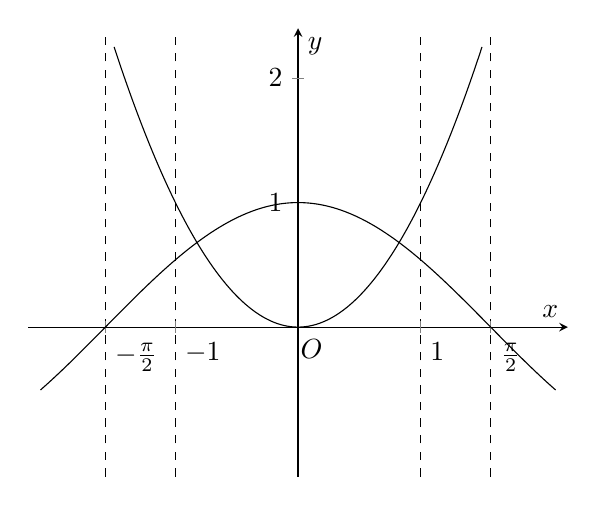
\begin{tikzpicture}
\begin{axis}
[
ymin=-1.2,ymax=2.4,
xmin=-2.2,xmax=2.2,
xtick=\empty,
ytick=\empty,
extra x ticks={-1.5708, -1, 1, 1.5708},
extra x tick labels={$-\frac{\pi}{2}$, $-1$, $1$, $\frac{\pi}{2}$},
extra y ticks={1, 2},
extra y tick labels={$1$, $2$},
every extra x tick/.style={
    xticklabel style={anchor=north west},
    grid=major,
    major grid style={very thin,dashed,black}
},
axis lines = center,
xlabel=$x$,ylabel=$y$,
samples=200,
]
\addplot [black, domain=-2.1:2.1] {cos(deg(x))};
\addplot [black, domain=-1.5:1.5] {x^2};
\node at (axis cs:0.11, -0.18) {$O$} ;
\end{axis}
\end{tikzpicture}
\end{document}
